\begin{pastexam}[label={px:ncku-112-prog-14}]{成大資訊聯招 112 學年度 第 14 題}
（計算）

(10\%) We are given a sequence $K=\langle k_1,k_2,\ldots,k_n\rangle$ of $n$ distinct keys in sorted order (so
that $k_1<k_2<\cdots<k_n$), and we wish to build a binary search tree from these keys. For each key $k_i$, we
have a probability $p_i$ that a search will be for $k_i$. Some searches may be for values not in $K$, and so
we also have $n+1$ ``dummy keys'' $d_0,d_1,\ldots,d_n$ representing values not in $K$. In particular, $d_0$
represents all values less than $k_1$, $d_n$ represents all values greater than $k_n$, and for
$i=1,2,\ldots n-1$, the dummy key $d_i$ represents all values between $k_i$ and $k_{i+1}$. For each dummy key
$d_i$, we have a probability $q_i$ that a search will correspond to $d_i$. Determine the cost and structure
of an optimal binary search tree in the expected cost of search time for a set of $n=7$ keys with the
following probabilities:
\begin{center}
\begin{tabular}{|c|c|c|c|c|c|c|c|c|}
\hline
$i$ & 0 & 1 & 2 & 3 & 4 & 5 & 6 & 7 \\ \hline
$p_i$ & & 0.04 & 0.06 & 0.08 & 0.02 & 0.10 & 0.12 & 0.14 \\ \hline
$q_i$ & 0.06 & 0.06 & 0.06 & 0.06 & 0.05 & 0.05 & 0.05 & 0.05 \\ \hline
\end{tabular}
\end{center}
\end{pastexam}

\begin{pastsoln}
答案：最小期望搜尋成本 $3.12$；根是 $k_5$，最佳樹如下（方框是虛擬鍵）。

照資結書第~18.4~節（CLRS 的寫法）。 期望成本是每個鍵和虛擬鍵的（深度 $+ 1$）乘上機率的和，也就是搜尋時
平均看幾個節點。 令 $e[i, j]$ 為用 $k_i, \ldots, k_j$（和 $d_{i-1}, \ldots, d_j$）建出的最佳子樹的期望成本，
$w(i, j) = \sum_{l=i}^{j} p_l + \sum_{l=i-1}^{j} q_l$ 是這棵子樹的總機率。 子樹接到別的節點下面時，每個節點深度
加 $1$，成本多 $w(i, j)$，所以
\[
e[i, j] = \begin{cases}
q_{i-1}, & j = i - 1,\\
\min_{i \le r \le j}\bigl(e[i, r-1] + e[r+1, j]\bigr) + w(i, j), & i \le j,
\end{cases}
\]
$\mathit{root}[i, j]$ 記下取到最小值的 $r$。 依區間長度由短到長填表，$w$ 用 $w(i, j) = w(i, j-1) + p_j + q_j$
遞推。

\textbf{$w(i, j)$}：
\begin{center}
\small
\begin{tabular}{c|cccccccc}
\toprule
$i \backslash j$ & 0 & 1 & 2 & 3 & 4 & 5 & 6 & 7 \\
\midrule
1 & 0.06 & 0.16 & 0.28 & 0.42 & 0.49 & 0.64 & 0.81 & 1.00 \\
2 &  & 0.06 & 0.18 & 0.32 & 0.39 & 0.54 & 0.71 & 0.90 \\
3 &  &  & 0.06 & 0.20 & 0.27 & 0.42 & 0.59 & 0.78 \\
4 &  &  &  & 0.06 & 0.13 & 0.28 & 0.45 & 0.64 \\
5 &  &  &  &  & 0.05 & 0.20 & 0.37 & 0.56 \\
6 &  &  &  &  &  & 0.05 & 0.22 & 0.41 \\
7 &  &  &  &  &  &  & 0.05 & 0.24 \\
8 &  &  &  &  &  &  &  & 0.05 \\
\bottomrule
\end{tabular}
\end{center}

\textbf{$e[i, j]$}：
\begin{center}
\small
\begin{tabular}{c|cccccccc}
\toprule
$i \backslash j$ & 0 & 1 & 2 & 3 & 4 & 5 & 6 & 7 \\
\midrule
1 & 0.06 & 0.28 & 0.62 & 1.02 & 1.34 & 1.83 & 2.44 & 3.12 \\
2 &  & 0.06 & 0.30 & 0.68 & 0.93 & 1.41 & 1.96 & 2.61 \\
3 &  &  & 0.06 & 0.32 & 0.57 & 1.04 & 1.48 & 2.13 \\
4 &  &  &  & 0.06 & 0.24 & 0.57 & 1.01 & 1.55 \\
5 &  &  &  &  & 0.05 & 0.30 & 0.72 & 1.20 \\
6 &  &  &  &  &  & 0.05 & 0.32 & 0.78 \\
7 &  &  &  &  &  &  & 0.05 & 0.34 \\
8 &  &  &  &  &  &  &  & 0.05 \\
\bottomrule
\end{tabular}
\end{center}

\textbf{$\mathit{root}[i, j]$}：
\begin{center}
\small
\begin{tabular}{c|ccccccc}
\toprule
$i \backslash j$ & 1 & 2 & 3 & 4 & 5 & 6 & 7 \\
\midrule
1 & $k_1$ & $k_2$ & $k_2$ & $k_2$ & $k_3$ & $k_3$ & $k_5$ \\
2 &  & $k_2$ & $k_3$ & $k_3$ & $k_3$ & $k_5$ & $k_5$ \\
3 &  &  & $k_3$ & $k_3$ & $k_4$/$k_5$ & $k_5$ & $k_5$ \\
4 &  &  &  & $k_4$ & $k_5$ & $k_5$ & $k_6$ \\
5 &  &  &  &  & $k_5$ & $k_6$ & $k_6$ \\
6 &  &  &  &  &  & $k_6$ & $k_7$ \\
7 &  &  &  &  &  &  & $k_7$ \\
\bottomrule
\end{tabular}
\end{center}
舉兩格示範。 $e[1, 2]$：$w(1, 2) = q_0 + p_1 + q_1 + p_2 + q_2 = 0.06 + 0.04 + 0.06 + 0.06 + 0.06 = 0.28$；$r = 1$ 時
$e[1, 0] + e[2, 2] = 0.06 + 0.30 = 0.36$，$r = 2$ 時 $e[1, 1] + e[3, 2] = 0.28 + 0.06 = 0.34$，取 $r = 2$，
$e[1, 2] = 0.34 + 0.28 = 0.62$。 $e[1, 7]$：$w(1, 7) = 1.00$，各個 $r$ 的 $e[1, r-1] + e[r+1, 7]$ 依序是
$0.06 + 2.61$、$0.28 + 2.13$、$0.62 + 1.55$、$1.02 + 1.20$、$1.34 + 0.78$、$1.83 + 0.34$、$2.44 + 0.05$，即
$2.67, 2.41, 2.17, 2.22, 2.12, 2.17, 2.49$，最小是 $r = 5$ 的 $2.12$，$e[1, 7] = 2.12 + 1.00 = 3.12$。
（$\mathit{root}[3, 5]$ 有 $k_4$、$k_5$ 兩個並列最佳，但這一格不在最後那棵樹的回推路徑上。）

\textbf{回推樹}。 $\mathit{root}[1, 7] = 5$：根 $k_5$，左子樹 $k_1..k_4$，右子樹 $k_6..k_7$。
$\mathit{root}[1, 4] = 2$：$k_2$，左 $k_1$，右 $k_3..k_4$；$\mathit{root}[3, 4] = 3$：$k_3$，右子 $k_4$。
$\mathit{root}[6, 7] = 7$：$k_7$，左子 $k_6$。
\begin{center}
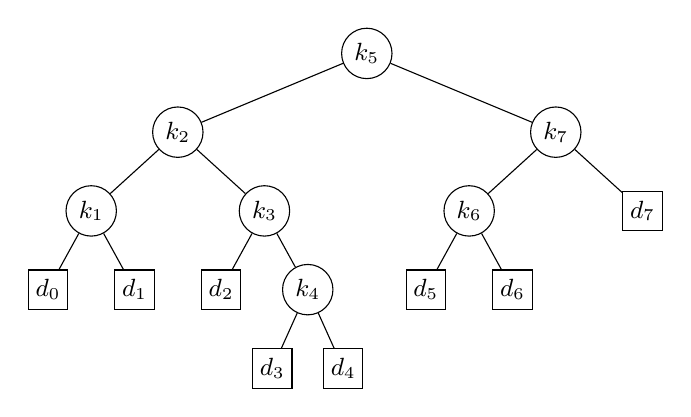
\begin{tikzpicture}[level distance=10mm,
  k/.style={circle,draw,inner sep=0pt,minimum size=6.4mm,font=\small},
  d/.style={rectangle,draw,inner sep=1pt,minimum size=5mm,font=\small},
  level 1/.style={sibling distance=48mm}, level 2/.style={sibling distance=22mm},
  level 3/.style={sibling distance=11mm}, level 4/.style={sibling distance=9mm}]
\node[k] {$k_5$}
  child {node[k] {$k_2$}
    child {node[k] {$k_1$} child {node[d] {$d_0$}} child {node[d] {$d_1$}}}
    child {node[k] {$k_3$} child {node[d] {$d_2$}}
      child {node[k] {$k_4$} child {node[d] {$d_3$}} child {node[d] {$d_4$}}}}}
  child {node[k] {$k_7$}
    child {node[k] {$k_6$} child {node[d] {$d_5$}} child {node[d] {$d_6$}}}
    child {node[d] {$d_7$}}};
\end{tikzpicture}
\end{center}
驗算：依深度（根為 $0$）算 $\sum (\text{深度} + 1) \times$ 機率：
\begin{itemize}
\item 深度 $0$：$k_5$，$1 \times 0.10 = 0.10$。
\item 深度 $1$：$k_2, k_7$，$2 \times (0.06 + 0.14) = 0.40$。
\item 深度 $2$：$k_1, k_3, k_6, d_7$，$3 \times (0.04 + 0.08 + 0.12 + 0.05) = 0.87$。
\item 深度 $3$：$d_0, d_1, d_2, k_4, d_5, d_6$，$4 \times (0.06 + 0.06 + 0.06 + 0.02 + 0.05 + 0.05) = 1.20$。
\item 深度 $4$：$d_3, d_4$，$5 \times (0.06 + 0.05) = 0.55$。
\end{itemize}
合計 $0.10 + 0.40 + 0.87 + 1.20 + 0.55 = 3.12$。
\end{pastsoln}
